\documentclass[12pt]{article}
\usepackage[round]{natbib}
\usepackage{graphicx}

\begin{document}

\section{Introduction}

\section{Method}

\subsection{Data}

The data set contains 660 mothers living in Mexico city.
They are all at least 18 years old,
and most of them are non-smokers.
All of them have singleton pregnancy and give live birth.
Each of them are examined by ultrasound for several times during pregnancy
and four parameters are measured:
head circumference (HC),
biparietal diameter (BPD),
abdominal circumference (AC),
and femur length (FL).
During pregnancy,
each mother is given a diet recommendation for each of five categories:
fruits,
legume,
red meat,
added sugar,
and purchased food that is high in saturated fat and sugar (HSFS).
In addition, biological and demographic parameters,
such as
baby's gender,
mother's body mass index,
and whether the mother is married,
are recorded.
For the details of the study population and design,
see \citet{o2013air}.
There are 548 mothers whose data is complete.
Since this is already 83\% of the whole data set,
we use the complete cases only in this analysis.

\subsection{Model}

\subsubsection{Measurement of Fetal Growth}

We need to decide on a measure for the size of the fetus.
This can be a single ultrasound parameter or a combination of more than one of them.
We observed that the four ultrasound parameters are highly correlated.
The Pearson correlation coefficients for HC vs. AC, BPD vs. AC, and FL vs. AC are all greater than 0.98.
This implies that any one of the four parameters is representative of the other three.
Thus we can choose a single parameter as our measure for fetal size.
Moreover, \citet{ott2002diagnosis} has shown that abdominal circumference is
very indictive of IUGR,
with a specificity of 90.7\% and sensitivity of 62.2\%.
The usefulness of AC in measuring fetal growth is also supported by
\citet{williams2001abdominal} and \cite{resnik2002intrauterine}.
Therefore, in this study we use AC as the measurement of fetal size.

\subsubsection{Selection of Covariates}

For measuring the mother's dietary quality,
we decide to use whether the mother meets the dietary recommendations.
We do not use the maternal dietary quality score because it does not tell us the effect of each kind of food.

For selecting the confounders,
we first did a literature review
for physiological and demographic variables that are commonly adjusted for
when studying external factors' effect on fetal growth.
\citet{smith2002early} in their study of plasma protein's association with IUGR,
as well as \citet{berkowitz2003world} and \citet{choi2008prenatal} in their studies of air pollution's association with IUGR,
include the baby's sex, mother's education level, parity, age, and BMI as confounders.
% sex 2, edu 1, age 2, parity 2, bmi 2,  height
Moreover, \citet{maisonet2004review} gave a literature review on air pollution's effect on fetal growth.
In their comparison of 5 separate studies on low birth weight and very low birth weight
\citep{
  alderman1987maternal,
  landgren1996environmental,
  bobak1999pregnancy,
  bobak2000outdoor,
  rogers2000association},
baby's sex, mother's education level, parity, and age
are common confounders that are adjusted for in more than one studies.
% sex 2, edu 3, age 3, parity 2, married, weight

Next, we explore our data set to find potential confounders.
For each mother,
we regress AC on weeks since LMP (with intercept).
The slope of this simple linear model is then regressed on each physiological and demographic variables in the data set.
As it turned out,
mother's age, parity, BMI, and average energy intake have a significant effect on AD (at $\alpha = 0.05$).

By combining the common practice in the literature
and the exploratory analysis of our data,
we decide to include baby's sex, mother's parity, age, and BMI as the confounders that need to be adjusted for.
Maternal education level is left out because it is not significant in our data and would increase the model complexity by adding 4 more categorical variables.
Pregancy average energy intake is not included as a confounder, either,
because it is closely related to the whether the mother meets the diet recommendations.

\subsubsection{Time Variable and Random Effects}

Finally, we fit a linear mixed model (LMM) to the data.
The time variable here is the weeks since LMP.
As the change of AC over time appear to follow a parabolic pattern,
we include a quadratic term for weeks since LMP.
Moreover, we allow the intercept to be random,
since the time between conception and LMP varies by individuals.
The coefficient of the linear term of weeks since LMP is also set to be random
to account for the different fetal size growth rate among individuals.
The quadratic term for time is not treated as random,
since when each baby's AC is regressed on quadratic time,
the coefficient for the quadratic term varies very little among individuals.

\section{Result}

\section{Discussion}

\newpage

\bibliographystyle{plainnat}
\bibliography{../699}

\appendix

\begin{figure}[p]
  \centering
  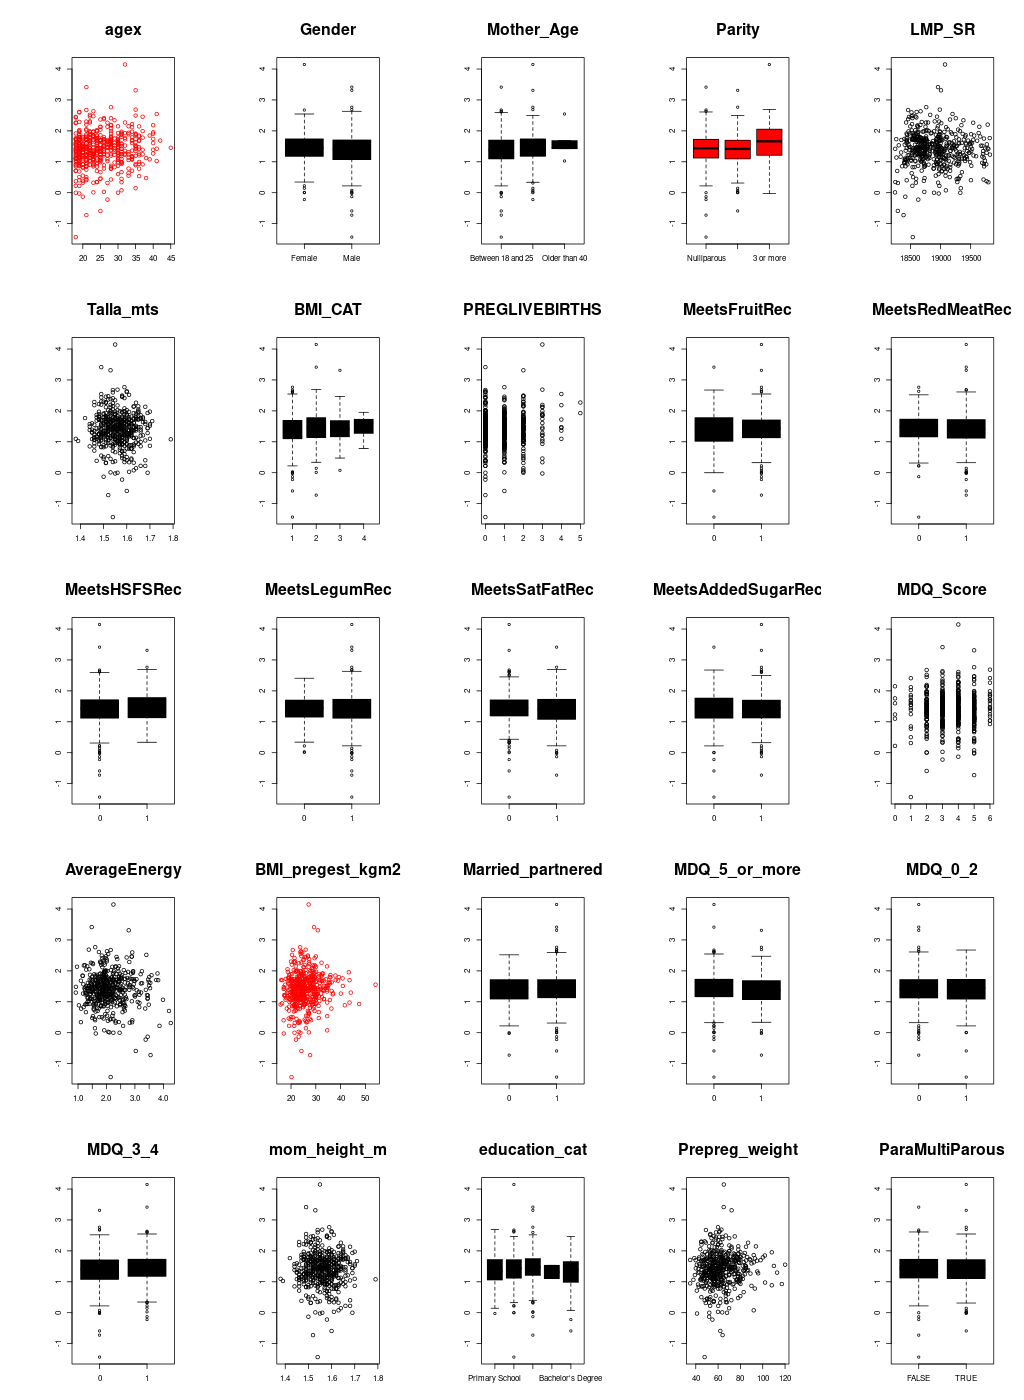
\includegraphics[width=0.98\textwidth]{cova}
  \caption{
    Individuals' AC growth slope regressed on each of the covariates.
    Covariates that has a significant effect on AC ($\alpha - 0.05$) are shown in red.
  }
  \label{fig:cova}
\end{figure}


\begin{figure}[p]
  \centering
  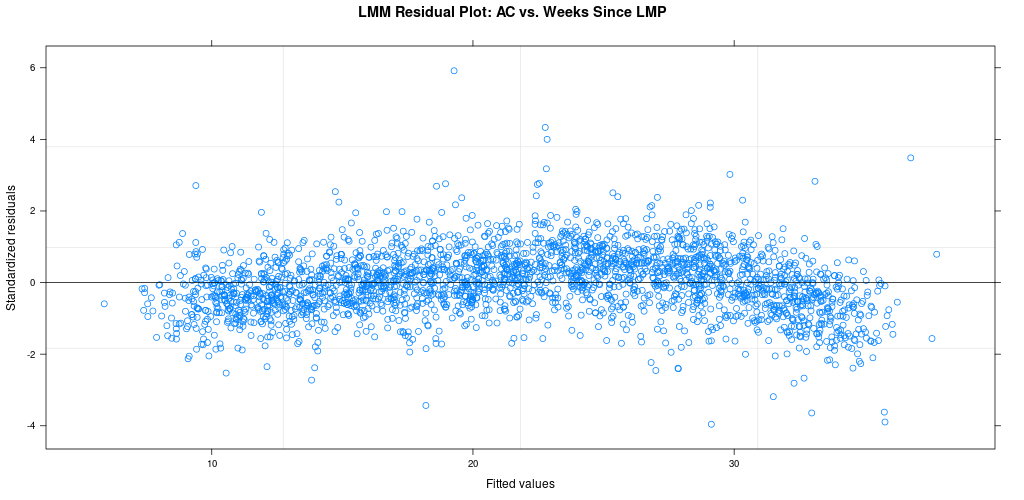
\includegraphics[width=0.98\textwidth]{lmm-lin}
  \caption{Residual plots without quadratic term.}
  \label{fig:lmm-lin}
\end{figure}


\begin{figure}[p]
  \centering
  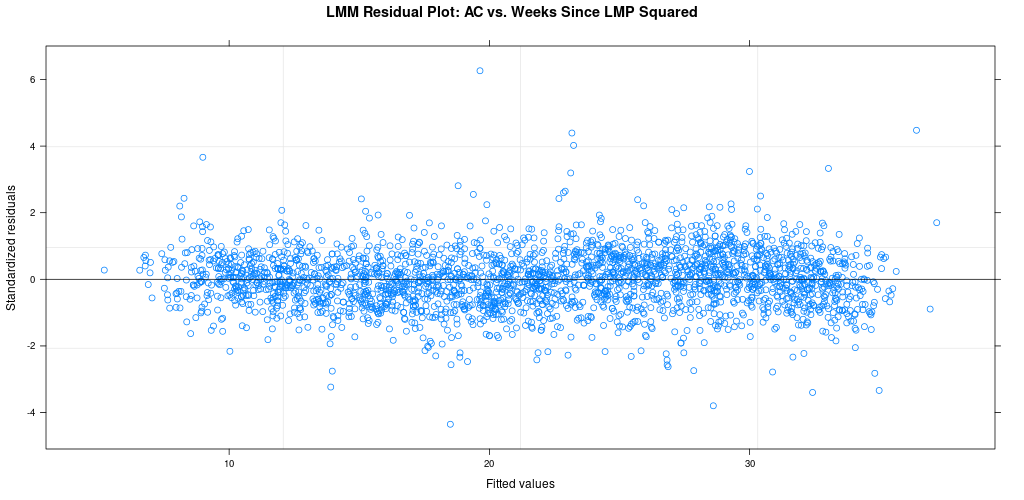
\includegraphics[width=0.98\textwidth]{lmm-qua}
  \caption{Residual plots with quadratic term.}
  \label{fig:lmm-qua}
\end{figure}

\end{document}